%% The lines that are not written within % .. % are not to be tampered with!!

\documentclass[twoside]{article}
\setlength{\oddsidemargin}{0.25 in}
\setlength{\evensidemargin}{-0.25 in}
\setlength{\topmargin}{-0.6 in}
\setlength{\textwidth}{6.5 in}
\setlength{\textheight}{8.5 in}
\setlength{\headsep}{0.75 in}
\setlength{\parindent}{0 in}
\setlength{\parskip}{0.1 in}

%
% ADD PACKAGES here:
\usepackage{amssymb}
\usepackage{multirow}

\usepackage[most]{tcolorbox} % 引入 tcolorbox 宏包
\usepackage{amsthm}
\usepackage{array}
\usepackage{booktabs}
\usepackage{xcolor}
\usepackage{amsmath,amsfonts,graphicx}
\usepackage{etoolbox} % 提供 \BeforeBeginEnvironment 和 \AfterEndEnvironment
\usepackage{graphicx}
\usepackage{tikz}
\tikzset{
    level distance=2cm,
    sibling distance=2.5cm
}

\newtheoremstyle{definitionstyle}
  {3pt}   % 上方间距
  {3pt}   % 下方间距
  {\normalfont} % 字体
  {}      % 缩进
  {\bfseries\color{blue}} % 标题字体
  {.}     % 标题后标点
  {0.5em} % 标题后间距
  {}      % 标题格式
\theoremstyle{definitionstyle}
\newtheorem*{definition}{Definition}
\newtheorem*{theorem}{Theorem}  
\BeforeBeginEnvironment{definition}{%
  \begin{tcolorbox}[
    colback=white,
    colframe=black,
    boxrule=0.6pt, % 边框粗细
    arc=0pt,       % 直角
    top=4pt,       % 上内边距
    bottom=4pt,    % 下内边距
    left=4pt,      % 左内边距
    right=4pt,     % 右内边距
    breakable,     % 允许跨页
  ]%
}
\AfterEndEnvironment{definition}{\end{tcolorbox}}

\BeforeBeginEnvironment{theorem}{
  \begin{tcolorbox}[
    colback=white,
    colframe=black,
    boxrule=0.6pt, % 边框粗细
    arc=0pt,       % 直角
    top=4pt,       % 上内边距
    bottom=4pt,    % 下内边距
    left=4pt,      % 左内边距
    right=4pt,     % 右内边距
    breakable,     % 允许跨页
  ]%
}
\AfterEndEnvironment{theorem}{\end{tcolorbox}}

\newcounter{lecnum}
\renewcommand{\thepage}{\thelecnum-\arabic{page}}
\renewcommand{\thesection}{\thelecnum.\arabic{section}}
\renewcommand{\theequation}{\thelecnum.\arabic{equation}}
\renewcommand{\thefigure}{\thelecnum.\arabic{figure}}
\renewcommand{\thetable}{\thelecnum.\arabic{table}}


\newcommand{\lecture}[4]{
   \pagestyle{myheadings}
   \thispagestyle{plain}
   \newpage
   \setcounter{lecnum}{#1}
   \setcounter{page}{1}
   \noindent
   \begin{center}
   \framebox{
      \vbox{\vspace{2mm}
    \hbox to 6.28in { {\bf MATH4321} }
       \vspace{4mm}
       \hbox to 6.28in { {\Large \hfill Lecture #1: #2  \hfill} }
       \vspace{2mm}
      \vspace{2mm}}
   }
   \end{center}
   \markboth{Lecture #1: #2}{Lecture #1: #2}
}



\renewcommand{\cite}[1]{[#1]}
\def\beginrefs{\begin{list}%
        {[\arabic{equation}]}{\usecounter{equation}
         \setlength{\leftmargin}{2.0truecm}\setlength{\labelsep}{0.4truecm}%
         \setlength{\labelwidth}{1.6truecm}}}
\def\endrefs{\end{list}}
\def\bibentry#1{\item[\hbox{[#1]}]}

%Use this command for a figure; it puts a figure in wherever you want it.
%usage: \fig{NUMBER}{SPACE-IN-INCHES}{CAPTION}
%This is for your help while typing the notes
\newcommand{\fig}[3]{
			\vspace{#2}
			\begin{center}
			Figure \thelecnum.#1:~#3
			\end{center}
	}

\newcommand\E{\mathbb{E}}
\newcommand{\PI}{$P_{i}$}
\newcommand{\KIA}{$K_{i}(A)$}
\newcommand{\FIW}{$F_{i}(\omega)$}
\newcommand{\OS}{$\omega ^{*}$}
\begin{document}
\lecture{3}{Games under incomplete information}{XIE}{}

\section{Games under incomplete information (Static Games)}
N-person static games under incomplete information(Bayesian games):\\
1. Set of players {1,2, … , N} \\
2.  Strategic set of players (denoted by $S_1, S_2, \ldots, S_N)$.\\
3. Type space of player (denoted by $\Theta_1, \Theta_2, \ldots, \Theta_N$). Each $\Theta_i = \{\underbrace{\theta_{i1}}_{type 1}, \underbrace{\theta_{i2}}_{type 2}, \ldots, \underbrace{\theta_{in_i}}_{type n_i}\}$ describes all possible types of player i.\\
4. Player i's belief on other players' types. Mathematically, it is quantified by the probability distribution which $p_i(\theta) = P(\theta_{-i} = \theta)$\\
5.  Player i's payoff function under various outcomes, which is type-dependent. We denote it by $v_i(s_i;s_{-i}; \theta_i)$.\\
Given a strategy $s_i(\theta_i)$ chosen by player i of type $\theta_i$ and the set of opponents'
strategies $s_{-i} = \{s_{-i}(\theta_{-i}):\theta_{-i}\in \Theta_{-i}\}$, the player i's expected payoff (her objective function) can be expressed as follows: 
$$V_i(s_i;s_{-i};\theta_i) = \sum_{\theta_{-i}\in\Theta_{-i}}\underbrace{p_i(\theta_{-i})}_{\text{P(opponents are of type }\theta_{-i})}\times v_i(s_i; s_{-i}(\theta_{-i}); \theta_i)$$\\
\begin{definition}[Bayesian Nash equilibrium]
    We say a strategic profile $s^* = (s_1^*, s_2^*, \ldots, s_N^*)$ is a Bayesian Nash equilibrium if and only if for any player i and any type $\theta_i$, we have 
\[ V_i(s_i^*(\theta_i); s_{-i}^*; \theta_i) \geq V_i(s; s_{-i}^*; \theta_i) \text{  for any }s\in S_i,\]
Here, $s_i^* = (s_i^*(\theta_{i1}), s_i^*(\theta_{i2}), \ldots, s_i^*(\theta_{in_i}))$ denotes the player i's strategies of different types. 
\end{definition}
\textbf{example:}\\
Two competing firms (firm 1 and firm 2) producing a common good for a market and each firm can choose the number of goods ($q_i$) produced. It is given that\\
1. The market price of the good is $p = 100 - q_1 - q_2$.\\
2. The production costs of two firms are $c_1 q_1$ and $c_2 q_2$ respectively. The true values of $c_1$ and $c_2$ are 10 and 10 respectively.\\
3. Firm 2 knows the production cost of firm 1 and Firm 1 does not know the exact production cost of firm2. Instead, Firm 1 knows that $c_2$ is either $c_2^L = 5$, $c_2^M = 10$ or $c_2^H = 20$ with probabilities $\frac{1}{3}$, $\frac{1}{3}$ and $\frac{1}{3}$ respectively.\\
Based on the above information, determine all possible Bayesian Nash equilibrium for this duopoly games.\\
\textbf{solution:} \\
We let $q_1$ be quantity chosen by Firm 1. We let $q_2^L = q_2(c_2^L)$, $q_2^M = q_2(c_2^M)$ and $q_2^H = q_2(c_2^H)$ be quantities chosen by different types of Firm 2. 

\paragraph{Step 1: Find the best response of Firm 1}
We first consider Firm 1's side. Given the strategies $(q_2^L, q_2^M, q_2^H)$ chosen by different types of Firm 2, the expected payoff of Firm 1 is expressed as 
\begin{align*}
V_1(q_1; q_2) &= \frac{1}{3} \times [(100 - q_1 - q_2^L)q_1 - 10q_1] + \frac{1}{3} \times [(100 - q_1 - q_2^M)q_1 - 10q_1] + \frac{1}{3} \times [(100 - q_1 - q_2^H)q_1 - 10q_1] \\
&= \dots = \left[ 90 - \frac{1}{3}q_2^L - \frac{1}{3}q_2^M - \frac{1}{3}q_2^H \right] q_1 - q_1^2.
\end{align*}
By considering the first-order condition, we have 
\[
\left. \frac{\partial V_1}{\partial q_1} \right|_{q_1 = q_1^*} = 0 \implies \left[ 90 - \frac{1}{3}q_2^L - \frac{1}{3}q_2^M - \frac{1}{3}q_2^H \right] - 2q_1^* = 0
\]
\[
\implies q_1^* = \frac{90 - \frac{1}{3}q_2^L - \frac{1}{3}q_2^M - \frac{1}{3}q_2^H}{2} \dots\dots (1).
\]

\paragraph{Step 2: Find the best response of Firm 2}
We proceed to determine the best response of Firm 2. Given Firm 1's strategy $q_1$ and the firm's type $c_{2i}$, the Firm 2's payoff is seen to be 
\[
V_2(q_{2i}; q_1, c_{2i}) = (100 - q_1 - q_{2i})q_{2i} - c_{2i}q_{2i}, \quad i = L, M, H.
\]
The best response can be found by considering the corresponding first order condition:
\[
\left. \frac{\partial V_2}{\partial q_{2i}} \right|_{q_{2i}^*} = 0 \implies (100 - c_{2i} - q_1) - 2q_{2i}^* = 0 \implies q_{2i}^* = \frac{100 - c_{2i} - q_1}{2}
\]
Substituting $c_{2i} = 5, 10$ and $20$, we get 
\[
q_2^{L*} = \frac{95 - q_1}{2}, \quad q_2^{M*} = \frac{90 - q_1}{2}, \quad q_2^{H*} = \frac{80 - q_1}{2} \dots\dots (2).
\]
Hence, the Bayesian Nash equilibrium can be identified by solving (1) and (2). Substitute (2) into (1), we get 
\[
q_1^* = \frac{90 - \frac{1}{3}\left(\frac{95 - q_1^*}{2}\right) - \frac{1}{3}\left(\frac{90 - q_1^*}{2}\right) - \frac{1}{3}\left(\frac{80 - q_1^*}{2}\right)}{2}
\]
\[
\implies q_1^* = 30.55556.
\]
From (2), we get 
\[
q_2^{L*} = \frac{95 - q_1^*}{2} = 32.2222, \quad q_2^{M*} = 29.7222, \quad q_2^{H*} = 24.7222.
\]
The corresponding actual profits made by two firms are given by 
\[
V_1 = (100 - 30.55556 - 29.7222)(30.55556) - 10(30.55556) \approx 908.179.
\]
\[
V_2(c_2^M) = (100 - 30.55556 - 29.7222)(29.7222) - 10(29.7222) \approx 883.4105.
\]
%
%
%
%
%
\textbf{example}:\\
Two universities offer two MSc. programs (Program A and B) and each MSc. program has only one vacancy. Peter (Player 1) and Ben (Player 2) are interested in applying MSc. program. Each of them can choose to apply one of these two programs. If they apply different program, they will be enrolled in their chosen program. If they apply the same program, they will compete and only one of them can get the offer and another will get nothing. We assume that Peter (player 1) can get the offer with probability $p$ ($p \in (0,1)$). The value of $p$ depends on Ben's (player 2) ability:
\begin{itemize}
    \item If Ben is better than Peter, then $p = 0.2$ (Peter has smaller chance to win).
    \item If Ben is worse than Peter, then $p = 0.7$ (Peter has larger chance to win).
\end{itemize}
It is given that the payoffs of enrolling into program A and program B are 5 and 2 respectively. Thus the player's (expected) payoff can then be described by the following matrix:

\begin{center}
    \begin{tabular}{rccc}
        & & \multicolumn{2}{c}{Player 2} \\
        & & A & B \\ \cline{3-4}
        Player 1 & A & \multicolumn{1}{|c|}{$(5p, 5(1 - p))$} & \multicolumn{1}{c|}{$(5,2)$} \\ \cline{3-4}
        & B & \multicolumn{1}{|c|}{$(2,5)$} & \multicolumn{1}{c|}{$(2p, 2(1 - p))$} \\ \cline{3-4}
    \end{tabular}
\end{center}

\noindent (a) Suppose that each player knows the ability of another player, find the Nash equilibrium for each value of $p$.\\
(b) We assume that Ben (player 2) knows Peter's (player 1) ability and Peter does not. Peter only knows that there is a probability $q$ that Ben is better than him.
\begin{itemize}
    \item[(i)] Take $q = 0.5$, find the Bayesian Nash equilibrium.
    \item[(ii)] Repeat the calculation for $q = 0.1$ and $q = 0.8$ and examine whether there is any difference in the final outcome of the games.
\end{itemize}

\textbf{solution(b)}:\\
Firstly, the Peter's belief on the value of $p$ is
\[
P(p = 0.2) = q, \quad P(p = 0.7) = 1 - q.
\]
To facilitate the later analysis, I will present the general procedure for finding BNE in this case.\\
We let $s_1$ and $s_2 = (s_{2L}, s_{2H})$ be the strategies of two players. Here, $s_{2L}$ denotes player 2's strategy when he knows $p = 0.2$ and $s_{2H}$ denotes player 2's when he knows $p = 0.7$

\subsection*{Step 1: Find the best response of player 2 (Ben)}
\begin{itemize}
    \item If Ben is of type $L$ (with $p = 0.2$), then the player 2's payoff matrix becomes
    \begin{center}
        \begin{tabular}{rccc}
            & & \multicolumn{2}{c}{Player 1} \\
            & & A & B \\ \cline{3-4}
            Player 2 $p = 0.2$ & A & \multicolumn{1}{|c|}{4} & \multicolumn{1}{c|}{5} \\ \cline{3-4}
            & B & \multicolumn{1}{|c|}{2} & \multicolumn{1}{c|}{1.6} \\ \cline{3-4}
            \textbf{Best response} & & A & A
        \end{tabular}
    \end{center}
    
    \item If Ben is of type $L$ (with $p = 0.2$), then the player 2's payoff matrix becomes
    \begin{center}
        \begin{tabular}{rccc}
            & & \multicolumn{2}{c}{Player 1} \\
            & & A & B \\ \cline{3-4}
            Player 2 $p = 0.7$ & A & \multicolumn{1}{|c|}{1.5} & \multicolumn{1}{c|}{5} \\ \cline{3-4}
            & B & \multicolumn{1}{|c|}{2} & \multicolumn{1}{c|}{0.6} \\ \cline{3-4}
            \textbf{Best response} & & B & A
        \end{tabular}
    \end{center}
\end{itemize}

\subsection*{Step 2: Find the best response of player 1 (Peter)}
Given the value of $q$ (belief), the expected payoff of player 1 under different strategic profile is given by

\begin{center}
    \small
    \begin{tabular}{ccccc}
        \toprule
        & \multicolumn{4}{c}{Player 2's strategy} \\
        & $(A, A)$ & $(A, B)$ & $(B, A)$ & $(B, B)$ \\
        \midrule
        A & $q + 3.5(1 - q) = 3.5 - 2.5q$ & $q + 5(1 - q) = 5 - 4q$ & $5q + 3.5(1 - q) = 3.5 + 1.5q$ & $5q + 5(1 - q) = 5$ \\
        \addlinespace
        B & $2q + 2(1 - q) = 2$ & $2q + 1.4(1 - q) = 0.6q + 1.4$ & $0.4q + 2(1 - q) = 2 - 1.6q$ & $0.4q + 1.4(1 - q) = 1.4 - q$ \\
        \midrule
        \textbf{Best response} & 
        $\begin{cases} A & \text{if } q = 0.1 \\ A & \text{if } q = 0.5 \\ B & \text{if } q = 0.8 \end{cases}$ & 
        $\begin{cases} A & \text{if } q = 0.1 \\ A & \text{if } q = 0.5 \\ B & \text{if } q = 0.8 \end{cases}$ & 
        A & 
        A \\
        \bottomrule
    \end{tabular}
\end{center}

\noindent Finally, we determine BNE by doing the following equilibrium analysis:

\begin{center}
    \small
    \begin{tabular}{cccc}
        \toprule
        Player 1's strategy & Player 2's strategy & Best response for player 1 & Best response for player 2 \\
        \midrule
        $A$ & $(A, A)$ & Yes if $q = 0.1$ Yes if $q = 0.5$ No if $q = 0.8$ & No \\
        & $(A, B)$ & Yes if $q = 0.1$ Yes if $q = 0.5$ No if $q = 0.8$ & Yes \\
        & $(B, A)$ & Yes & No \\
        & $(B, B)$ & Yes & No \\
        \midrule
        $B$ & $(A, A)$ & No if $q = 0.1$ No if $q = 0.5$ Yes if $q = 0.8$ & Yes \\
        & $(A, B)$ & No if $q = 0.1$ No if $q = 0.5$ Yes if $q = 0.8$ & No \\
        & $(B, A)$ & No & No \\
        & $(B, B)$ & No & No \\
        \bottomrule
    \end{tabular}
\end{center}

\noindent Therefore, we conclude that
\begin{itemize}
    \item When $q = 0.1$, the BNEs will be $(s_1, s_2) = [A, (A, B)]$.
    \item When $q = 0.5$, the BNEs will be $(s_1, s_2) = [A, (A, B)]$.
    \item When $q = 0.8$, the BNEs will be $(s_1, s_2) = [B, (A, A)]$.
\end{itemize}
Generally speaking, Peter consider to apply program $B$ (yielding lower payoff) if he has strong belief that Ben is stronger than him (i.e. $q$ is very high).\\
\newline
%
%
%
%
%
\textbf{example:}\\
There are two bidders in a second price sealed-bid auction. It is given that \\
1. The true valuations of bidder 1 and 2 are $v_1 = 60$ and $v_2 = 65$; \\
2. Bidder 1 conjectures that bidder 2’s valuation has the following probability distribution 
    \[
    P(v_2 = 55) = P(v_2 = 65) = P(v_2 = 75) = \frac{1}{3}.
    \]
3. Bidder 2 knows the exact value of bidder 1’s valuation $v_1 = 60$. \\
(a) Find the best responses of each bidder. \\
(b) Hence, find a (not all) Bayesian Nash equilibrium for this bidding games. (*Note: It will be very tedious to determine all Bayesian Nash equilibria)

\textbf{Solution of (a)} \\
We first obtain the best response of bidder 2 (denoted by $b_{2j}^*$, $j = L, M, H$) of different types. Given the bid $b_1$ submitted by bidder 1, the bidder 2’s payoff can be expressed as 
\[
V_2(b_{2j}; b_1, v_{2j}) = \mathbf{1}_{\{b_{2j} < b_1\}}(0) + \mathbf{1}_{\{b_{2j} = b_1\}}\left\{\frac{1}{2}(v_{2j} - b_1)\right\} + \mathbf{1}_{\{b_{2j} > b_1\}}(v_{2j} - b_1).
\]
We consider the following 3 cases:

\vspace{0.5em}
\noindent \textbf{Case 1a: If $v_{2j} > b_1$,} \\
The bidder 2 can gain the winning status and enjoy a largest payoff $v_{2j} - b_1$ by submitting any bid strictly higher than $b_1$ (i.e. $b_{2j} > b_1$). So the best response is determined to be $b_{2j}^* \in (b_1, \infty)$.

\vspace{0.5em}
\noindent \textbf{Case 1b: If $v_{2j} = b_1$,} \\
The bidder 2 gets zero payoff whenever he wins or loses the games. Thus the best response is $b_{2j}^* \in [0, \infty)$.

\vspace{0.5em}
\noindent \textbf{Case 1c: If $v_{2j} < b_1$,} \\
The bidder 2 will get a negative payoff $v_{2j} - b_1 < 0$ if he submits a bid higher than $b_1$. The corresponding best response is $b_{2j}^* \in [0, b_1)$ (Here, bidder 2 will lose the games).

\vspace{0.5em}
\noindent Next, we determine the best response of bidder 1. \\
Given the bids $b_2(\cdot) = (b_{2L}, b_{2M}, b_{2H})$ submitted by different types of bidder 2, the expected payoff of bidder 1 can be expressed as 
\begin{align*}
V_1(b_1; b_2(\cdot), v_1) &= \sum_{j \in \{L,M,H\}} P(v_2 = v_{2j}) \left\{\mathbf{1}_{\{b_1 < b_{2j}\}}(0) + \mathbf{1}_{\{b_1 = b_{2j}\}}\left\{\frac{1}{2}(v_1 - b_{2j})\right\} + \mathbf{1}_{\{b_1 > b_{2j}\}}(v_1 - b_{2j})\right\} \\
&= \sum_{j \in \{L,M,H\}} \frac{1}{3}\left\{\mathbf{1}_{\{b_1 < b_{2j}\}}(0) + \mathbf{1}_{\{b_1 = b_{2j}\}}\left\{\frac{1}{2}(v_1 - b_{2j})\right\} + \mathbf{1}_{\{b_1 > b_{2j}\}}(v_1 - b_{2j})\right\}.
\end{align*}
To obtain the best response of bidder 1, we consider the following three cases:

\vspace{0.5em}
\noindent \textbf{Case 2a: If $\max(b_{2L}, b_{2M}, b_{2H}) < v_1$,} \\
Bidder 1 can maximize his payoff by submitting any bid higher than $\max(b_{2L}, b_{2M}, b_{2H})$ since raising the bid can increase the chance of winning without harming the final payoff (why??). So the best response is $b_1^* \in (\max(b_{2L}, b_{2M}, b_{2H}) , \infty)$.

\vspace{0.5em}
\noindent \textbf{Case 2b: If $\max(b_{2L}, b_{2M}, b_{2H}) > v_1 > \min(b_{2L}, b_{2M}, b_{2H})$} \\
We consider the case when $b_{2L} < b_{2M} < v_1 < b_{2H}$ (the derivation of other cases is similar). Note that bidder 1 should get a negative payoff will be resulted if the bidder 2 is of type $H$ ($v_2 = v_{2H}$) as $v_1 - b_{2H} < 0$. \\
On the other hand, the bidder 1's payoff is maximized if it submits a bid higher than $b_{2M}$ (why). Thus the best response will be $b_1^* \in (b_{2M}, b_{2H})$. \\
(*Remark: In general, the bidder 1's best response is to submit a bid within $(\max_{j: b_{2j} < v_1} b_{2j}, \min_{j: b_{2j} > v_1} b_{2j})$.)

\vspace{0.5em}
\noindent \textbf{Case 2c: If $\min(b_{2L}, b_{2M}, b_{2H}) > v_1$} \\
Since $v_1 - b_{2j} < 0$ for all $i = L, M, H$, the negative payoff will be resulted if the bidder 1 chooses to offer a bid higher than $\min(b_{2L}, b_{2M}, b_{2H})$, so bidder 1 will lose the games for sure and the best responses will be $b_1^* \in [0, \min(b_{2L}, b_{2M}, b_{2H}))$.

\vspace{1em}
\noindent \textbf{Solution of (b)} \\
A careful observation shows that submitting a bid that equal to the valuation (i.e. $b_i^* = v_i$) is always the best response of player $i$ with respect to the opponent’s strategy. Hence, one possible Bayesian Nash equilibrium will be that all players submit the bid that equal to their own valuation. That is, 
\[
b_1^* = v_1, \qquad b_{2j}^* = v_{2j}, \dots \quad (*)
\]
where $j = L, M, H$. \\
We first verify the optimality of bidder 2. 
\begin{itemize}
    \item If the bidder 2 is of type $L$ (with $v_2 = v_{2L} = 55$), he will submit a bid $b_{2L}^* = v_2 = 55$. Given that $b_1^* = v_1 = 60$, the result in case 1(c) reveals that the bidder 2’s best response is any bid within $[0,60)$. This implies that $b_{2L}^*$ is the best response to $b_1^*$. 
    \item If the bidder 2 is of type $M$ (with $v_2 = v_{2M} = 65$), he will submit a bid $b_{2M}^* = v_2 = 65$. Given that $b_1^* = v_1 = 60$, the result in case 1(a) reveals that the bidder 2’s best response is any bid within $[60, \infty)$. This implies that $b_{2M}^*$ is the best response to $b_1^*$. 
    \item If the bidder 2 is of type $H$ (with $v_2 = v_{2H} = 75$), one can apply the similar analysis in previous case and deduce that $b_{2H}^* = v_{2H} = 75$ is the best response to $b_1^* = 60$. 
\end{itemize}
Next, we proceed to verify the optimality of bidder 1. Given that $b_{2L}^* = 55$, $b_{2M}^* = 65$ and $b_{2H}^* = 75$, the result in case 2(b) reveals that the best response of bidder 1 is to submit a bid within $(55,65)$. So $b_1^* = 60$ is the best response to bidder 2’s strategy. \\
Hence, we conclude that the strategic profile defined in $(*)$ is the Bayesian Nash equilibrium.
\begin{theorem}
    In a second price auction games, there is a Bayesian Nash equilibrium in 
which all players bid at their true valuations. That is $b_i^*(v_i) = v_i$ for any player i and any type $v_i$. 
\end{theorem}
proof: Given the opponent's strategy, the expected payoff of bidder i is seen to be 
\[
V_1(b_1^*; b_{-1}^*, v_1) = V_1(v_1; v_{-1}, v_1) 
\]
\[
= \sum_{j=1}^M P(\text{Opponent's valuation is } v_{2j}) \left\{ \mathbf{1}_{\{b_1 < \max_{j \neq 1} v_{2j}\}}(0) + \mathbf{1}_{\{b_1 = \max_{j \neq 1} v_{2j}\}} \left\{ \frac{1}{n}(v_1 - \max_{j \neq 1} v_{2j}) \right\} + \mathbf{1}_{\{b_1 > \max_{j \neq 1} v_{2j}\}} (v_1 - \max_{j \neq 1} v_{2j}) \right\}.
\]
where n is number of players submitting the highest bid.  \\
\text{***}\\
for a First price sealed-bid auction under incomplete information, we deduce that the symmetric Bayesian Nash equilibrium is given by 
\[
b(v_i) = v_i - \frac{\int_{\underline{v}}^{v_i} [F(v_i)]^{N-1} dv_i}{[F(v_i)]^{N-1}}
\]




\section{Games under incomplete information (Dynamic Games)}

\textbf{Updating player's belief over the game - Bayes' Rule} \\
We consider a player $i$ which has $m$ possible types (denoted by $\theta_{i1}, \theta_{i2}, \dots, \theta_{im}$ respectively). We let \\
1. $p_j(\theta_{ik}) = P(\theta_i = \theta_{ik})$ be the player $j$'s belief on player $i$'s type and \\
2. $s_i(\theta_{ik})$ be the pure strategy (or mixed strategy in general) chosen by player $i$ of type $k$.\\
Suppose that player $j$ observes that player $i$ has chosen a strategy $A \in S_i$, then player $j$'s updated belief can be estimated as
\[
p_j(\theta_{ik}|A) = P(\theta_i = \theta_{ik}|A) = \frac{P(\theta_i = \theta_{ik} \text{ and } A)}{P(A)} = \frac{P(A|\theta_i = \theta_{ik})p_j(\theta_{ik})}{\sum_{k=1}^m P(A|\theta_i = \theta_{ik})p_j(\theta_{ik})}.
\]
The above formula is also known as Bayes' rule. \\
(*Note: $P(A|\theta_i = \theta_{ik}) = 0$ or $1$ if player $i$ adopts pure strategy.)

\begin{definition}[Belief System]
    A system belief $\mu$ of a dynamic games assigns a probability distribution over 
decision nodes to every information set. That is, for every information set h and for every decision node x, $\mu (x|h)$ denotes the probability that the player is at node $x \in h$. In addition, $\sum_{x\in h}\mu(x|h) = 1$ for every information set h. 
\end{definition}
For other information set that are off the equilibrium path, the Bayes' rule cannot be applied. In the case, any belief can be assigned. (*Note: In equilibrium analysis, we will set the off-the-equilibrium path in such a way that the players have no incentive to deviate from on-the-equilibrium path)\\
Given the belief system $\mu$, we expect that the players' strategies must be sequentially rational in the sense that in every information set h, the players will choose a strategy which is a best response to their beliefs and the rival's strategy. 
That is, given the rival’s strategy $s_{-i}$, the player $i$ chooses the strategy $s_i^*$ such that

$$\underbrace{\mathbb{E}[ v_i( s_i^*; s_{-i} , \theta_i ) \mid \mu , h ]}_{\substack{\text{Expected payoff} \\ \text{(given belief and} \\ \text{information set})}} \ge \mathbb{E}[v_i(s_i; s_{-i}, \theta_i) \mid \mu, h] \quad \text{for any } s_i \in S_i \dots \dots (*)$$

for any information set $h$.
\begin{definition}[Perfect Bayesian Equilibrium]
    A strategic profile $s^* = (s_1^*, s_2^*, \ldots, s_n^*)$ and a belief system $\mu$ constitute Perfect 
Bayesian Equilibrium if and only if 
\begin{itemize}
\item Players' strategies are sequentially rational which the inequality (*) holds for all players. 
\item The belief system $\mu$ that are on-the equilibrium path should be determined according to strategic profile and Bayes' rule. 
\end{itemize}
\end{definition}
obtain the PBE of a dynamic games:\\
1. By Ad-hoc searching\\
- Step 1: Obtain all Bayesian Nash equilibrium (BNE) by definition.\\
- Step 2: For each BNE, we construct the corresponding belief system.\\
- Step 3: Check the sequential rationality of players.\\
2: By Backward induction\\
At each step, we obtain the optimal strategies of the players for every possible updated belief. 
Then, we determine the optimal strategies and the belief system that is consistent to proposed optimal strategies.\\
\newline
%
%
%
\textbf{example:}\\
There are two players in the games: Player 1 is a potential entrant to an industry and Player 2 is an incumbent who is monopolistic in this industry.\\
1. Player 1 first decides whether it will enter the industry ($E$) or will not enter the industry ($NE$). The game ends if player 1 chooses not enter the industry.\\
2. If player 1 decides to enter the industry, player 2 (incumbent) will decide either fight against the entry ($F$) or accommodate the entry ($A$). The game ends afterwards.\\
We assume that the incumbent does not know the competitiveness of the entrant. Instead, it conjectures that the entrant is competitive (type $C$) with probability $p$ and is weak (type $W$) with probability $1 - p$. The entrant knows its type.

\textbf{Payoff structure}:\\
1. If the entrant does not enter into the industry, the incumbent will receive a payoff of 4 and the entrant receives nothing.\\
2. If the entrant enters into the industry, the players' payoff, which depends on the entrant's type and the incumbent's strategy, is summarized as follows:\\
\begin{center}
\begin{tabular}{r|cc}
    & Competitive ($C$) & Weak ($W$) \\ \hline
    Fight ($F$) & $(-1, -1)$ & $(-2, 3)$ \\
    Accommodate ($A$) & $(2, 2)$ & $(-1, 2)$
\end{tabular}
\end{center}

Then we determine all Bayesian Nash equilibrium of the games by taking $p = \frac{1}{2}$.

\textbf{Step 1: Find the best response of player 1}:\\
\begin{itemize}
    \item If player 1 is of type $C$, then the payoff matrix is given as follows:
    \begin{center}
    \begin{tabular}{r|cc}
        \multicolumn{1}{c}{} & \multicolumn{2}{c}{Player 2} \\
        Player 1 & $F$ & $A$ \\ \hline
        $E$ & $(-\mathbf{1}, -1)$ & $(\mathbf{2}, 2)$ \\
        $NE$ & $(\mathbf{0}, 4)$ & $(\mathbf{0}, 4)$
    \end{tabular}
    \end{center}
    Then the best response of player 1 is:
    $$s_1^*(C) = \begin{cases} 
    NE & \text{if } s_2 = F \\ 
    E & \text{if } s_2 = A 
    \end{cases}$$

    \item If player 1 is of type $W$, then the payoff matrix is given as follows:
    \begin{center}
    \begin{tabular}{r|cc}
        \multicolumn{1}{c}{} & \multicolumn{2}{c}{Player 2} \\
        Player 1 & $F$ & $A$ \\ \hline
        $E$ & $(-\mathbf{2}, 3)$ & $(-\mathbf{1}, 2)$ \\
        $NE$ & $(\mathbf{0}, 4)$ & $(\mathbf{0}, 4)$
    \end{tabular}
    \end{center}
    Then the best response of player 1 is:
    $$s_1^*(W) = \begin{cases} 
    NE & \text{if } s_2 = F \\ 
    NE & \text{if } s_2 = A 
    \end{cases}$$
\end{itemize}
\textbf{Step 2: Find the best response of player 2}:\\
Given his belief, player 2's expected payoff under different strategic profiles can be computed as:

\begin{center}
\begin{tabular}{c|cc}
    Player 1's strategy $s_1 = (s_1(C), s_1(W))$ & $A$ & $F$ \\ \hline
    $(E, E)$ & $\frac{1}{2}(2) + \frac{1}{2}(2) = \mathbf{2}$ & $\frac{1}{2}(-1) + \frac{1}{2}(3) = \mathbf{1}$ \\
    $(E, NE)$ & $\frac{1}{2}(2) + \frac{1}{2}(4) = \mathbf{3}$ & $\frac{1}{2}(-1) + \frac{1}{2}(4) = \mathbf{1.5}$ \\
    $(NE, E)$ & $\frac{1}{2}(4) + \frac{1}{2}(2) = \mathbf{3}$ & $\frac{1}{2}(4) + \frac{1}{2}(3) = \mathbf{3.5}$ \\
    $(NE, NE)$ & $\frac{1}{2}(4) + \frac{1}{2}(4) = \mathbf{4}$ & $\frac{1}{2}(4) + \frac{1}{2}(4) = \mathbf{4}$
\end{tabular}
\end{center}

By comparing the payoffs, player 2's best response is found to be:
$$s_2^* = \begin{cases}
A & \text{if } s_1 = (E, E) \\
A & \text{if } s_1 = (E, NE) \\
F & \text{if } s_1 = (NE, E) \\
A \text{ or } F & \text{if } s_1 = (NE, NE)
\end{cases}$$

\textbf{Step 3: Determine the Bayesian Nash equilibrium}:\\
\begin{center}
\begin{tabular}{cc|cc}
    $s_1$ & $s_2$ & Best response for player 1? & Best response for player 2? \\ \hline
    $(E, E)$ & $F$ & No & No \\
             & $A$ & No & Yes \\ \hline
    $(E, NE)$ & $F$ & No & No \\
              & $A$ & Yes & Yes \\ \hline
    $(NE, E)$ & $F$ & No & Yes \\
              & $A$ & No & No \\ \hline
    $(NE, NE)$ & $F$ & Yes & Yes \\
               & $A$ & No & Yes
\end{tabular}
\end{center}

We conclude from the above table that the Bayesian Nash equilibria are $(s_1^*, s_2^*) = ((E, NE), A)$ or $(s_1^*, s_2^*) = ((NE, NE), F)$.

\begin{enumerate}
    \item[(a)] Determine if $(s_1^*, s_2^*) = ((E, NE), A)$ constitutes the Perfect Bayesian Equilibrium (PBE).
    \item[(b)] Determine if $(s_1^*, s_2^*) = ((NE, NE), F)$ constitutes the PBE.
\end{enumerate}

\textbf{Solution(method 1)}:\\
\textbf{(a)} We first determine the belief system of player 2 (the only player who does not know the type of another player).

If the players adopt the equilibrium $s_1^* = (E, NE)$ and $s_2^* = A$:
\begin{itemize}
    \item If player 1 chooses $E$, then player 2's belief is given by:
    $$\underbrace{p_2(C \mid E)}_{\mu(x_1(2))} = \frac{1(p)}{1(p) + 0(1 - p)} \overset{p=0.5}{=} 1, \qquad \underbrace{p_2(W \mid E)}_{\mu(x_2(2))} = \frac{0(1 - p)}{1(p) + 0(1 - p)} \overset{p=0.5}{=} 0$$
    
    \item If player 1 chooses $NE$, then the corresponding belief is given by:
    $$p_2(C \mid NE) = \frac{0(p)}{0(p) + 1(1 - p)} \overset{p=0.5}{=} 0, \qquad p_2(W \mid NE) = \frac{1(1 - p)}{0(p) + 1(1 - p)} \overset{p=0.5}{=} 1$$
\end{itemize}
\textit{(*Note: Player 1 knows its own type and there is no uncertainty on player 2's belief, so it is not necessary to define the belief of player 1.)}

Next, we proceed to check the sequential rationality of each player.
\begin{itemize}
    \item \textbf{We first consider player 2.} Note that player 2's belief is $p_2(C \mid E) = 1$ and $p_2(W \mid E) = 0$ if player 1 chooses $E$. It follows that:
    $$\mathbb{E}[v_2(A; s_1^*) \mid \mu, h] = \underbrace{p_2(C \mid E)}_{=1} \underbrace{v_2(A; E, C)}_{=2} + \underbrace{p_2(W \mid E)}_{=0} \underbrace{v_2(A; E, W)}_{=2} = 2$$
    $$\mathbb{E}[v_2(F; s_1^*) \mid \mu, h] = \underbrace{p_2(C \mid E)}_{=1} \underbrace{v_2(F; E, C)}_{=-1} + \underbrace{p_2(W \mid E)}_{=0} \underbrace{v_2(F; E, W)}_{=3} = -1$$
    Since $\mathbb{E}[v_2(A; s_1^*) \mid \mu, h] > \mathbb{E}[v_2(F; s_1^*) \mid \mu, h]$, $s_2^* = A$ is sequentially rational.

    \item \textbf{Next, we consider player 1.} Since player 1 knows that player 2 will choose $A$ if it chooses to enter into the industry, it follows that:
    \begin{itemize}
        \item If player 1 is of type $C$ and $s_1^*(C) = E$, we have:
        $$v_1(E; A, C) = 2 > 0 = v_1(NE; A, C)$$
        \item If player 1 is of type $W$ and $s_1^*(W) = NE$, we have:
        $$v_1(NE; A, W) = 0 > -1 = v_1(E; A, W)$$
    \end{itemize}
    So player 1 (of any type) has no incentive to deviate and its strategy is also sequentially rational. Therefore, $((E, NE), A)$ constitutes a PBE.
\end{itemize}

\textbf{(b)} Next, we consider the strategic profile $(s_1^*, s_2^*) = ((NE, NE), F)$ and determine the belief system for player 2:
\begin{itemize}
    \item If player 1 chooses $NE$, then the corresponding belief is given by:
    $$p_2(C \mid NE) = \frac{1(p)}{1(p) + 1(1 - p)} \overset{p=0.5}{=} \frac{1}{2}, \qquad p_2(W \mid NE) = \frac{1(1 - p)}{1(p) + 1(1 - p)} \overset{p=0.5}{=} \frac{1}{2}$$
    
    \item If player 1 chooses $E$, the belief cannot be defined using Bayes' rule since it is on an off-the-equilibrium path. So we write:
    $$p_2(C \mid E) = q, \qquad p_2(W \mid E) = 1 - q$$
    where $q \in [0,1]$ is some constant.
\end{itemize}

Suppose that player 1 has chosen $E$ and $s_2^* = F$. One can verify that:
$$\mathbb{E}[v_2(F; s_1^*) \mid \mu, h] = \underbrace{p_2(C \mid E)}_{=q} \underbrace{v_2(F; E, C)}_{=-1} + \underbrace{p_2(W \mid E)}_{=1-q} \underbrace{v_2(F; E, W)}_{=3} = 3 - 4q$$
$$\mathbb{E}[v_2(A; s_1^*) \mid \mu, h] = \underbrace{p_2(C \mid E)}_{=q} \underbrace{v_2(A; E, C)}_{=2} + \underbrace{p_2(W \mid E)}_{=1-q} \underbrace{v_2(A; E, W)}_{=2} = 2$$

Note that:
$$\mathbb{E}[v_2(F; s_1^*) \mid \mu, h] \ge \mathbb{E}[v_2(A; s_1^*) \mid \mu, h] \iff 3 - 4q \ge 2 \iff q \le \frac{1}{4}$$
By choosing the off-the-equilibrium belief with some $q \le \frac{1}{4}$, player 2 has no incentive to deviate.

Finally, we consider player 1. Since player 1 knows that player 2 will choose $F$ if it chooses to enter into the industry, it follows that:
\begin{itemize}
    \item If player 1 is of type $C$ and $s_1^*(C) = NE$, we have:
    $$v_1(NE; F, C) = 0 > -1 = v_1(E; F, C)$$
    \item If player 1 is of type $W$ and $s_1^*(W) = NE$, we have:
    $$v_1(NE; F, W) = 0 > -2 = v_1(E; F, W)$$
\end{itemize}
Thus, player 1 also has no incentive to deviate. Therefore, $((NE, NE), F)$ constitutes a PBE supported by any off-the-equilibrium belief $q \le \frac{1}{4}$.\\
\newline
\textbf{Solution(method 2)}:\\
We will first determine the optimal strategy of player 2. 
We let $\mu(E) = (q, 1 - q)$ be player 2’s updated belief on player 1’s type if he knows player 1 chose $E$. Recall that:
\begin{itemize}
    \item The expected payoff of choosing $F$ is $(-1)q + 3(1 - q) = 3 - 4q$;
    \item The expected payoff of choosing $A$ is $2q + 2(1 - q) = 2$.
\end{itemize}
Hence, we conclude that player 2 will play $F$ if $3 - 4q \ge 2 \iff q \le \frac{1}{4}$ and play $A$ if $3 - 4q \le 2 \iff q \ge \frac{1}{4}$.

Next, we determine player 1’s optimal strategy. We consider 2 cases:

\paragraph{Case 1: $q \le \frac{1}{4}$ and player 2 plays $F$ if player 1 chooses $E$}
Then the optimal strategy of player 1 will be $s_1(C) = NE$ ($0$ vs. $-1$) if player 1 is of type $C$, and $s_1(W) = NE$ ($0$ vs. $-2$) if player 1 is of type $W$ respectively.

Since player 1 never chooses $E$, the updated player 2’s belief when player 1 chooses $E$ can be arbitrary ($q$ can be any number from 0 to 1) since it is a belief on the off-the-equilibrium path. By choosing $q \le \frac{1}{4}$ on the off-the-equilibrium path, the strategic profile $((NE, NE), F)$ is a PBE.

\paragraph{Case 2: $q \ge \frac{1}{4}$ and player 2 plays $A$ if player 1 chooses $E$}
Then the optimal strategy of player 1 will be $s_1(C) = E$ ($0$ vs. $2$) if player 1 is of type $C$, and $s_1(W) = NE$ ($0$ vs. $-1$) if player 1 is of type $W$ respectively.

If player 1 chooses $E$, then player 2 knows that player 1 must be of type $C$ so that the corresponding belief is $\mu(E) = (p_2(C), p_2(W)) = (1, 0)$, which corresponds to $q = 1$.

Since player 2’s optimality is consistent with the belief system, we conclude that the strategic profile $((E, NE), A)$ is a PBE.

\vspace{0.5em}
\noindent\textit{*Note: Since player 2’s updated belief cannot be determined until player 1’s strategy is known, this is the reason why we need to determine player 2’s optimal strategy for any possible belief when using backward induction.}
%
%
%
\begin{theorem}
    We let $s^* = (s_1^*, s_2^*, \ldots, s_n^*)$ be a Bayesian Nash equilibrium of a dynamic games. Suppose that the strategic profile $s^*$ induces that 
    every information node can be reached with a positive probability, then $s^*$ and the belief system $\mu^*$ derived uniquely from $s^*$ by Bayes' rule constitutes the Perfect Bayesian Equilibrium.
\end{theorem}
%
%
%
\textbf{example(Signaling Games):}\\
In this example, we shall investigate the signaling value of education. That is, whether acquiring a professional qualification can convey a “positive message” to employers so that the candidate can receive a better job offer.

There are 2 people in this game: Graduate Student (Player 1) and Employer (Player 2).
\begin{itemize}
    \item The student (Player 1) just graduated from his UG study and wishes to pursue a career in a certain industry. The student decides whether to pursue an additional professional qualification before getting the job ($Q$) or apply for the job immediately without pursuing the qualification ($N$).
    \begin{itemize}
        \item Getting the qualification requires some effort that is type-dependent: The cost will be $c_H = 2$ if the student has high productivity (Type H) and will be $c_L = 5$ if the student has low productivity (Type L). We assume that the student knows his own type.
    \end{itemize}
    \item The student applies for the job afterwards. After knowing the student’s qualification, the employer (Player 2) can assign the student to be either a manager ($M$) or a trainee ($T$). It is given that the market wage for a manager is $w_M = 10$ and the market wage for a trainee is $w_T = 6$.
    \item However, the employer does not know the actual productivity of the student at the time when he gives the offer to the student. Instead, the employer conjectures that there is a probability $p = 0.25$ that the student has high productivity and the probability that the student has low productivity is $0.75$.
    \item Player 2’s payoff (i.e., profit made by the employer) is determined by the combination of the student's productivity and the job assignment. The payoffs are summarized in the following payoff matrix:
\end{itemize}

\begin{center}
\begin{tabular}{r|cc}
    \multicolumn{1}{c}{} & \multicolumn{2}{c}{Player 2's decision} \\
    Productivity & $M$ & $T$ \\ \hline
    $H$ & 10 & 5 \\
    $L$ & 0 & 3
\end{tabular}
\end{center}

On the other hand, the payoff of the student (player 1) is simply the wage received minus the cost required for acquiring the professional qualification. (Note: The cost will be 0 if the student decides not to get the qualification.)

Determine all Perfect Bayesian Nash equilibria of the game.

\vspace{1em}
\noindent\textbf{Solution}

Firstly, one can draw the game tree as follows:

% Insert your uploaded image file name here
\begin{center}
    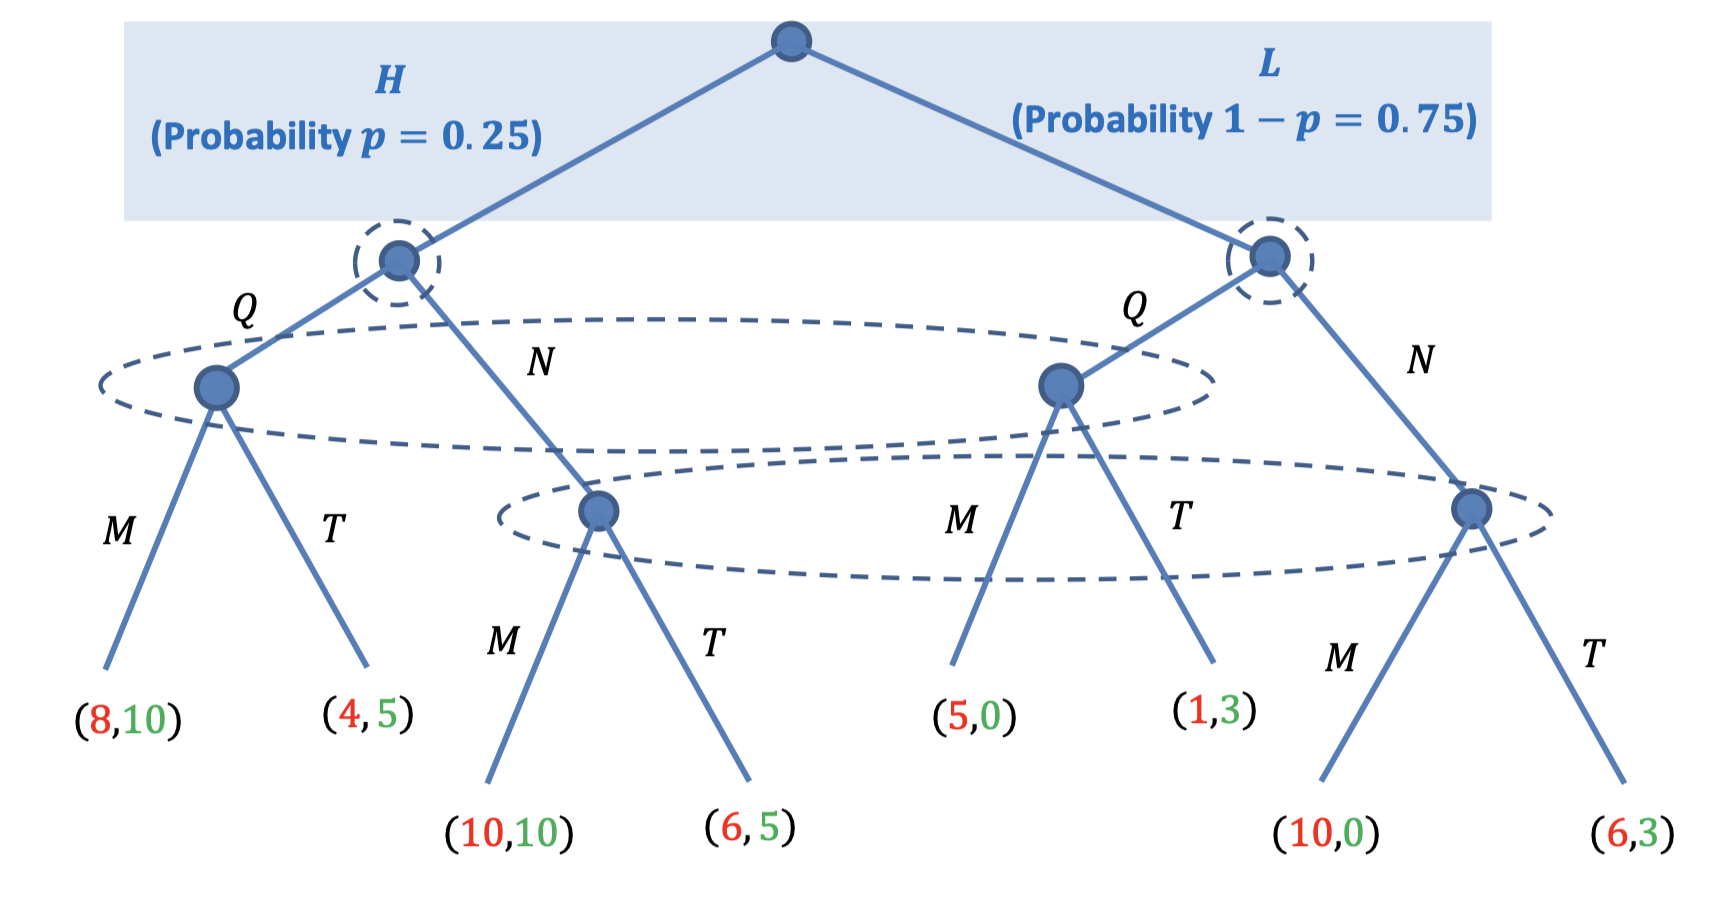
\includegraphics[width=0.9\textwidth]{Screenshot 2026-05-22 at 20.26.59.png}
\end{center}

We let $s_1^* = (s_{1H}, s_{1L})$ and $s_2^* = (s_{2Q}, s_{2N})$ be the strategic profile of player 1 and player 2 (at different information nodes). Here, $s_{1k}$ denotes player 1’s strategy given that he is of type $k \in \{H, L\}$ and $s_{2j}$ denotes player 2’s strategy if he observes that player 1 plays $j \in \{Q, N\}$.

We proceed to find the Perfect Bayesian Equilibrium using backward induction: We let $\mu(Q) = (q_Q, 1 - q_Q)$ and $\mu(N) = (q_N, 1 - q_N)$ be player 2’s updated beliefs when player 1 plays $Q$ and plays $N$ respectively.

\vspace{0.5em}
\noindent\textbf{Find the best response of player 2}

If player 1 plays $Q$, then the expected payoffs of playing $M$ and $T$ are given by:
$$\mathbb{E}[v_2(M; Q)] = (10)q_Q + (0)(1 - q_Q) = 10q_Q$$
$$\mathbb{E}[v_2(T; Q)] = (5)q_Q + (3)(1 - q_Q) = 3 + 2q_Q$$
Since $\mathbb{E}[v_2(M; Q)] \ge \mathbb{E}[v_2(T; Q)] \iff 10q_Q \ge 3 + 2q_Q \iff q_Q \ge \frac{3}{8}$, so we deduce that player 2 should play $M$ if $q_Q \ge \frac{3}{8}$ and play $T$ if $q_Q < \frac{3}{8}$.

\vspace{0.5em}
\noindent If player 1 plays $N$, then the expected payoffs of playing $M$ and $T$ are given by:
$$\mathbb{E}[v_2(M; N)] = (10)q_N + (0)(1 - q_N) = 10q_N$$
$$\mathbb{E}[v_2(T; N)] = (5)q_N + (3)(1 - q_N) = 3 + 2q_N$$
Since $\mathbb{E}[v_2(M; N)] \ge \mathbb{E}[v_2(T; N)] \iff 10q_N \ge 3 + 2q_N \iff q_N \ge \frac{3}{8}$, so we deduce that player 2 should play $M$ if $q_N \ge \frac{3}{8}$ and play $T$ if $q_N < \frac{3}{8}$.

\vspace{0.5em}
\noindent\textbf{Find the best response of player 1}

Next, we determine player 1’s optimal strategy given player 2’s best response. Using the game tree provided, player 1’s payoffs under player 2’s strategies are summarized as follows:

\begin{center}
\textbf{Type H} \\
\begin{tabular}{c|cccc}
    & $s_2^* = (M, M)$ & $s_2^* = (M, T)$ & $s_2^* = (T, M)$ & $s_2^* = (T, T)$ \\ \hline
    $Q$ & 8 & 8 & 4 & 4 \\
    $N$ & 10 & 6 & 10 & 6 \\ \hline
    \textbf{Best response} & \textbf{N} & \textbf{Q} & \textbf{N} & \textbf{N}
\end{tabular}
\end{center}

\begin{center}
\textbf{Type L} \\
\begin{tabular}{c|cccc}
    & $s_2^* = (M, M)$ & $s_2^* = (M, T)$ & $s_2^* = (T, M)$ & $s_2^* = (T, T)$ \\ \hline
    $Q$ & 5 & 5 & 1 & 1 \\
    $N$ & 10 & 6 & 10 & 6 \\ \hline
    \textbf{Best response} & \textbf{N} & \textbf{N} & \textbf{N} & \textbf{N}
\end{tabular}
\end{center}

\vspace{0.5em}
\noindent\textbf{Determine the Bayesian Nash equilibrium}

We consider the following four cases:

\vspace{0.5em}
\noindent\textbf{Case 1: If $s_2^* = (M, M)$ (when $q_Q \ge \frac{3}{8}$ and $q_N \ge \frac{3}{8}$)} \\
Then the best response of player 1 is $s_1^* = (N, N)$ and the corresponding player 2’s belief with respect to $s_1^*$ is:
$$\mu(Q) = (q, 1 - q), \qquad \mu(N) = (0.25, 0.75)$$
Here, $q$ can be any number between 0 and 1. \\
Since $q_N = 0.25 \le \frac{3}{8}$, there is no PBE when $s_2^* = (M, M)$.

\vspace{0.5em}
\noindent\textbf{Case 2: If $s_2^* = (M, T)$ (when $q_Q \ge \frac{3}{8}$ and $q_N < \frac{3}{8}$)} \\
Then the best response of player 1 is $s_1^* = (Q, N)$ and the corresponding player 2’s belief with respect to $s_1^*$ is:
$$\mu(Q) = (1,0), \qquad \mu(N) = (0, 1)$$
Since $q_Q = 1 \ge \frac{3}{8}$ and $q_N = 0 < \frac{3}{8}$, the belief system is consistent and $(s_1^*, s_2^*) = ((Q, N), (M, T))$ is a PBE.

\vspace{0.5em}
\noindent\textbf{Case 3: If $s_2^* = (T, M)$ (when $q_Q < \frac{3}{8}$ and $q_N \ge \frac{3}{8}$)} \\
Then the best response of player 1 is $s_1^* = (N, N)$ and the corresponding player 2’s belief with respect to $s_1^*$ is:
$$\mu(Q) = (q, 1 - q), \qquad \mu(N) = (0.25, 0.75)$$
Since $q_N = 0.25 \le \frac{3}{8}$, there is no PBE when $s_2^* = (T, M)$.

\vspace{0.5em}
\noindent\textbf{Case 4: If $s_2^* = (T, T)$ (when $q_Q < \frac{3}{8}$ and $q_N < \frac{3}{8}$)} \\
Then the best response of player 1 is $s_1^* = (N, N)$ and the corresponding player 2’s belief with respect to $s_1^*$ is:
$$\mu(Q) = (q, 1 - q), \qquad \mu(N) = (0.25, 0.75)$$
Since $q_N = 0.25 < \frac{3}{8}$, the updated belief will be consistent if $q < \frac{3}{8}$. Thus, $(s_1^*, s_2^*) = ((N, N), (T, T))$ is also a PBE.

\vspace{0.5em}
\noindent\textbf{Conclusion} \\
We conclude that there are 2 PBEs in this game:
\begin{enumerate}
    \item The separating equilibrium: $(s_1^*, s_2^*) = ((Q, N), (M, T))$ supported by beliefs $\mu(Q)=(1,0)$ and $\mu(N)=(0,1)$.
    \item The pooling equilibrium: $(s_1^*, s_2^*) = ((N, N), (T, T))$ supported by beliefs $\mu(N)=(0.25,0.75)$ and any off-equilibrium belief $\mu(Q)=(q, 1-q)$ where $q < \frac{3}{8}$.
\end{enumerate}
There are three possible types of equilibrium (PBE) in a signaling games.\\
1. Separating Equilibrium\\
Under this equilibrium, player 1 of different types adopt different strategies. That is, $s_1(\theta_{1j})\neq s_1(\theta_{1k})$ for any $\theta_{1j}\neq\theta_1k$. Then the player 2 can completely figure out the true type of player 1 by observing the strategy chosen by player 1.\\
2. Pooling Equilibrium\\
Under this equilibrium, player 1 of all types will adopt a common strategy. That is, $s_1(\theta_1) = s^*$ for all $\theta_1\in \Theta_1$. In this case, the player 2 fails to update his/her belief on player 1's type by observing the strategy.\\
3. Semi-pooling Equilibrium\\
Under this equilibrium, some types of player 1 will choose a common strategy and other types of player 1 will choose other different strategy. In this scenario, the player 2 may be able to obtain partial/complete information on player 1's type by observing player 1's action.\\
\newline
intuitive criterion: aims to examine if some types of players have incentive to deviate from a given equilibrium strategy and adopt the strategy in off-the-equilibrium path.\\
\newline
For any non-empty subset $T \subseteq \Theta_1$, we let $BR(T, a_1)$ be the set of all pure-strategy best responses for player 2 to player 1’s action $a_1$ for all beliefs $\mu = (p_2(\theta_{11} \mid a_1), p_2(\theta_{12} \mid a_1), \dots, p_2(\theta_{1n_1} \mid a_1))$ such that $\sum_{\theta_1 \in T} p_2(\theta_1 \mid a_1) = 1$. That is,
$$BR(T, a_1) = \bigcup_{\mu: \sum_{\theta_1 \in T} p_2(\theta_1 \mid a_1)=1} BR(\mu, a_1)$$
where
$$BR(\mu, a_1) = \operatorname{argmax}_{a_2} \underbrace{\sum_{\theta_1 \in \Theta_1} p_2(\theta_1 \mid a_1) v_2(a_2; a_1, \theta_1)}_{\text{Expected payoff of player 2 (updated belief)}}$$

\begin{definition}[Intuitive Criterion]
    We let $s_1^* = (s_1^*(\theta_{11}), s_1^*(\theta_{12}), \dots, s_1^*(\theta_{1n_1}))$ and $s_2^*$ be the equilibrium strategies of player 1 and player 2 in a signaling game.

We say the equilibrium fails the intuitive criterion if and only if there exists a strategy $a_1 \in S_1$ (which belongs to the off-equilibrium path) and a set of types $J(a_1) \subset \Theta_1$ such that:

\begin{enumerate}
    \item Player 1 of type $\theta_1 \in J(a_1)$ has no incentive to deviate from the equilibrium and play $a_1$, regardless of player 2’s updated belief when he observes player 1 play $a_1$:
    $$v_1(s_1^*(\theta_1); s_2^*, \theta_1) > \max_{a_2 \in BR(\Theta_1, a_1)} v_1(a_1; a_2, \theta_1) \quad \text{for all } \theta_1 \in J(a_1)$$
    
    \item There exists a type $\theta_1' \in \Theta_1$ such that player 1 of type $\theta_1'$ has an incentive to deviate to $a_1$ given that player 2 believes player 1’s type $\theta_1 \in \Theta_1 \setminus J(a_1)$ if player 1 chooses $a_1$. That is,
    $$v_1(s_1^*(\theta_1'); s_2^*, \theta_1') < \underbrace{\min_{a_2 \in BR(\Theta_1 \setminus J(a_1), a_1)} v_1(a_1; a_2, \theta_1')}_{\substack{\text{Minimum payoff} \\ \text{(deviate and play } a_1\text{)}}}$$
\end{enumerate}
\end{definition}

\textbf{example}: \\
We revisit the signaling game in Example 7. Recall that there are two PBEs in the game, namely:
$$(s_1^*, s_2^*) = ((Q, N), (M, T))$$
$$(s_1^{**}, s_2^{**}) = ((N, N), (T, T))$$

\begin{enumerate}
    \item[(a)] Argue that the pooling equilibrium $(s_1^{**}, s_2^{**}) = ((N, N), (T, T))$ fails the intuitive criterion.
    \item[(b)] Determine if the separating equilibrium $(s_1^*, s_2^*)$ satisfies the intuitive criterion.
\end{enumerate}

\vspace{1em}
\noindent\textbf{Solution of (a)}

It suffices to argue that there exists a player type who has an incentive to deviate and choose $Q$ (the only strategy other than $N$).

We take $a_1 = Q$, $J(a_1) = \{L\}$, and $\theta_1' = H$ in the intuitive criterion. We obtain:
\begin{itemize}
    \item For any $\theta_1 \in J(a_1)$ (i.e., $\theta_1 = L$):
    $$v_1(s_1^{**}(\theta_1); s_2^{**}, \theta_1) = v_1(N; (T, T), L) = 6$$
    $$\max_{a_2 \in BR(\Theta_1, a_1)} v_1(a_1; a_2, \theta_1) = \max_{a_2 \in BR(\Theta_1, Q)} v_1(Q; a_2, L) = \max(5, 1) = 5$$
    So we have $v_1(s_1^{**}(\theta_1); s_2^{**}, \theta_1) > \max_{a_2 \in BR(\Theta_1, a_1)} v_1(a_1; a_2, \theta_1)$.
    
    \item For player 1 of type $\theta_1' = H$, we get:
    $$v_1(s_1^{**}(\theta_1'); s_2^{**}, \theta_1') = v_1(N; (T, T), H) = 6$$
    $$\min_{a_2 \in BR(\Theta_1 \setminus J(a_1), a_1)} v_1(a_1; a_2, \theta_1') = \min_{a_2 \in BR(\{H\}, Q)} v_1(Q; a_2, H) \overset{a_2=M \text{ (why?)}}{=} v_1(Q; M, H) = 8$$
    So we deduce that $v_1(s_1^{**}(\theta_1'); s_2^{**}, \theta_1') < \min_{a_2 \in BR(\Theta_1 \setminus J(a_1), a_1)} v_1(a_1; a_2, \theta_1')$.
\end{itemize}
Therefore, the pooling equilibrium fails the intuitive criterion.


\textbf{Solution of (b)}

Since there is no off-the-equilibrium path under this separating equilibrium (i.e., all information nodes are reached with a positive probability), the separating equilibrium automatically satisfies the intuitive criterion.


\subsection*{Problems}
\textbf{1.}
We consider the following market entry game. There are $N$ firms ($N \geq 2$) and each firm can decide whether to enter a common market. The revenue of entering the market is $\frac{P}{n}$, where $n$ is the number of firms entering the market and $P > 0$ is a fixed constant. It is given that:\\
1. The entering cost of firm $i$ is $c_i$.\\
2. The value of $c_i$ is the private information for firm $i$, and other firms know that $c_i$ follows a uniform distribution over the interval $(0, C]$. We assume that $P > C$.\\

\noindent \textbf{(a) (10 marks)} Show that for firm $i$, there exists a threshold $\hat{c}_i$ such that firm $i$ will enter the market if and only if $c_i \leq \hat{c}_i$.\\
\noindent \textbf{(b) (10 marks)} Using (a), prove that there exists a symmetric Bayesian Nash equilibrium such that all firms adopt the same strategy, i.e., $s_1^*(c) = s_2^*(c) = \dots = s_N^*(c) = s^*(c)$. Here $s_i^*(c)$ denotes firm $i$'s strategy if its entering cost is $c_i = c$.\\
\noindent \textbf{Solution to (a):}\\
\noindent For any firm $i$ with entering cost $c_i$, we first examine the criterion on which the firm will enter the market. We consider the following two scenarios:\\
1. If the firm chooses not to enter the market, the payoff will be $0$.
2. If the firm chooses to enter the market, the expected payoff is seen to be:
    \[
    \sum_{k=0}^{N-1} \mathbb{P}\left(\text{$k$ of other $N-1$ firms enter the market}\right) \cdot \frac{P}{k+1} - c_i
    \]
Hence, the firm will enter the market if and only if:
\[
\sum_{k=0}^{N-1} \mathbb{P}\left(\text{$k$ of other $N-1$ firms enter the market}\right) \cdot \frac{P}{k+1} - c_i \geq 0
\]
\[
\iff c_i \leq \underbrace{\sum_{k=0}^{N-1} \mathbb{P}\left(\text{$k$ of other $N-1$ firms enter the market}\right) \cdot \frac{P}{k+1}}_{\hat{c}_i}
\]
Therefore, the strategic profile of firm $i$ can be characterized as a cutoff strategy follows:
\[
s_i^*(c) = 
\begin{cases} 
\text{Enter } (E) & \text{if } c \leq \hat{c}_i \\ 
\text{Not Enter } (NE) & \text{if } c > \hat{c}_i 
\end{cases}
\]












\end{document}